\documentclass[5p,times,authoryear=false]{elsarticle}
\usepackage[T1]{fontenc}
\usepackage{amsmath,amssymb,amsthm}
\usepackage{graphicx}
\usepackage{booktabs}
\usepackage{multirow}
\usepackage{xcolor}
\usepackage{algorithm}
\usepackage{algpseudocode}
\usepackage[hidelinks]{hyperref}
\usepackage{microtype}
\graphicspath{{figures/}}
\newtheorem{proposition}{Proposition}
\biboptions{numbers,sort&compress}

\journal{Future Generation Computer Systems}

\begin{document}
\begin{frontmatter}

\title{FedCAST: Budget-Aware Federated Stream Clustering over Apache Kafka under Non-IID Data and Network Constraints}

\author[1]{Author One}
\author[1]{Author Two}
\author[1]{Author Three}
\affiliation[1]{organization={Department of Computer Science, University Name},city={City},country={Country}}

\begin{abstract}
Edge devices produce unlabeled, non-IID data streams over constrained and heterogeneous links, yet operators need a continuously updated global clustering without collecting raw data. We present FedCAST, a budget-aware federated stream clustering system built on Apache Kafka. Each node summarises its stream with time-decayed cluster features and decides, at every tick, whether an update is worth its network cost and which micro-clusters to send. The decision uses an objective-linked staleness score that provably bounds the coordinator's k-means cost error and centroid displacement. A knapsack-style prioritisation, a scale-free exponentiated dual-ascent threshold, a token bucket with a hard budget guarantee, a link-price term, and a novelty override for clusters seen at a single node complete the policy. The coordinator aggregates staleness-decayed summaries with warm-started weighted k-means and swap local search, which protects node-exclusive clusters. Kafka's per-key ordering, idempotent producers and log-compacted changelog provide exactly-once state and crash recovery without resends, and the complete system runs in under 1\,GB of RAM. Across five datasets, seven baselines, non-IID partitions, drift, heterogeneous links and more than 2{,}000 seeded runs, FedCAST reaches within 5\,\% of a centralised learner's clustering cost with 10--61\,\% fewer bytes than the best baseline and up to 8.5$\times$ fewer than periodic synchronisation. It ranks first at matched budgets (Friedman $p{=}2{\times}10^{-4}$) and detects emerging clusters 2.5$\times$ faster than periodic updates while sending less. On a real broker it recovers from a coordinator crash in about one second with state identical to an uninterrupted run and loses no update during a broker outage.
\end{abstract}


\begin{keyword}
federated clustering \sep data streams \sep communication efficiency \sep non-IID data \sep Apache Kafka \sep edge computing
\end{keyword}
\end{frontmatter}

\section{Introduction}\label{sec:intro}

Network probes, industrial gateways, smart meters and vehicles continuously produce unlabeled data streams at the edge. Operators want a single, continuously updated \emph{global} view of the structure in these streams, such as the traffic profiles present in a network right now or the operating regimes of a machine fleet. Three obstacles stand in the way. First, raw data often cannot leave the device, for regulatory, privacy or volume reasons. Second, the data are \emph{non-IID}: each device sees a different slice of the global distribution, and some patterns are visible at a single device only. Third, links are constrained and heterogeneous: metered cellular uplinks, lossy wireless and intermittent connectivity make every transmitted byte costly.

Stream clustering answers the first obstacle with compact micro-cluster summaries~\cite{aggarwal2003clustream,cao2006denstream}. Distributed variants ship these summaries to a coordinator~\cite{cormode2007divide,gama2011dgclust,tran2013communication}, and federated clustering handles heterogeneity on static data~\cite{dennis2021kfed,zhang2025afcl}. What is missing is a principled answer to the question every edge node faces at every instant: \emph{is sending an update now worth its network cost, and if so, which part of the model should be sent?} Existing systems answer with a fixed period or a data-unit threshold. Periodic updates waste bytes when nothing changes and leave the server stale exactly when the data drift. Thresholds must be re-tuned for every dataset, and neither is connected to the quality of the global clustering or to a byte budget.

This paper presents \textbf{FedCAST}, a federated stream clustering system in which every byte is spent where it reduces the global clustering error most, within a hard per-node budget, on top of Apache Kafka. Our contributions are:
\begin{enumerate}
\item \textbf{Objective-linked staleness.} A per-micro-cluster score computed on the device from CF vectors and the broadcast global model. Its sum provably bounds the server's k-means cost error (Proposition~\ref{prop:cost}) and the displacement of the global centres (Proposition~\ref{prop:centroid}).
\item \textbf{A budgeted, prioritised, link-aware send policy.} Knapsack-style selection of the most valuable micro-clusters, a scale-free exponentiated dual-ascent threshold, a token bucket with a hard guarantee and $O(1/n)$ long-run convergence (Proposition~\ref{prop:budget}), a link-price term, and a novelty override for clusters that appear at a single node.
\item \textbf{Heterogeneity-aware aggregation.} Staleness-decayed, optionally node-balanced weighted k-means over CFs with swap local search, which keeps node-exclusive clusters from being absorbed by warm-started centres.
\item \textbf{A Kafka-native system.} Per-key ordering, idempotent producers with sequence numbers, and a compacted changelog give exactly-once state and crash recovery without any resend from the nodes. The complete system runs in under 1\,GB of RAM.
\item \textbf{A rigorous evaluation} on five datasets with seven baselines, five non-IID regimes, drift, heterogeneous links and outages, more than 2{,}000 seeded runs, and real-broker fault-injection experiments.
\end{enumerate}

To reach within 5\,\% of a centralised learner's clustering cost, FedCAST needs 10--61\,\% fewer bytes than the best baseline on every dataset and up to 8.5$\times$ fewer than periodic synchronisation. At matched budgets it ranks first ($p{=}2{\times}10^{-4}$, Friedman). It detects emerging clusters 2.5$\times$ faster than periodic updates while sending less. It recovers from a coordinator SIGKILL in about 1\,s with state identical to an uninterrupted run, and loses no update during a 34\,s broker outage.

\section{Related work}\label{sec:related}

\paragraph{Stream clustering} The two-phase paradigm, online micro-clusters followed by offline macro-clustering, was introduced by CluStream~\cite{aggarwal2003clustream}, building on BIRCH's cluster features~\cite{zhang1996birch}. DenStream~\cite{cao2006denstream} added exponential decay and density-based macro-clustering, and DBSTREAM~\cite{hahsler2016dbstream} a shared-density graph; see~\cite{zubaroglu2021review} for a survey. FedCAST uses decayed CFs as its unit of exchange because they are additive, cheap to send, and give the k-means cost in closed form, which is what makes an objective-linked trigger computable on the device.

\paragraph{Distributed stream clustering} Cormode et al.~\cite{cormode2007divide} maintain a continuous k-center clustering over distributed streams with approximation guarantees. DGClust~\cite{gama2011dgclust} sends grid-cell state changes from sensors, and Tran and Sattler~\cite{tran2013communication} send micro-clusters from remote sites to a coordinator. These works reduce communication with fixed, objective-agnostic rules (state change, period or threshold). They have no byte budget, do not adapt to link conditions, do not treat statistical heterogeneity, and are evaluated in simulation without a messaging substrate. Coreset-based methods~\cite{balcan2013distributed} offer strong guarantees for static data but no cheap incremental delta.

\paragraph{Federated clustering} k-FED~\cite{dennis2021kfed} performs one-shot federated k-means and shows that heterogeneity \emph{helps} when each device holds few clusters. FFCM~\cite{stallmann2022ffcm} federates fuzzy c-means, and AFCL~\cite{zhang2025afcl} handles asynchrony and an unknown number of clusters. All of them assume static local datasets. We run k-FED periodically as a strong baseline and report the regimes in which it wins.

\paragraph{Federated learning on streams} FedCluLearn~\cite{angelova2025fedclulearn} uses micro-cluster indexing to fight forgetting in federated continual \emph{supervised} learning. Silva et al.~\cite{silva2022federated} and DFAS~\cite{li2025dfas} address federated anomaly detection on streams. None of these targets clustering of the data itself under an explicit communication budget.

\paragraph{Event-triggered and communication-efficient learning} Communication efficiency is central in federated learning~\cite{mcmahan2017fedavg,kairouz2021advances}. Event-triggered schemes send when the norm of a parameter change exceeds a threshold, possibly adapted to device resources~\cite{ghosh2021eventgrad,zehtabi2022event}. FedCAST differs in three ways: its trigger is measured in the clustering objective and bounds the server's error (Propositions~\ref{prop:cost} and~\ref{prop:centroid}); it enforces a byte budget with a guarantee (Proposition~\ref{prop:budget}); and it prioritises \emph{which} parts of the model to send.

\paragraph{Kafka for federated ML} Kafka-ML~\cite{martin2022kafkaml} and its federated extension~\cite{carnerero2024kafkaml} use Kafka as the data and model transport for neural-network training. In FedCAST, Kafka's ordering, idempotence, replay and compaction semantics are part of the algorithm's recovery and exactly-once-state argument, and we measure them under crashes.

\section{Problem formulation}\label{sec:problem}

\paragraph{Setting} A set of $m$ edge nodes observes unlabeled streams. Node $i$ receives points $x\in\mathbb{R}^d$ drawn from a time-varying local distribution $P_i(t)$, and the local distributions are non-IID: $P_i\neq P_j$, and a cluster may be observed by a single node only. The network-wide distribution is the mixture $P(t)=\sum_i \pi_i(t)P_i(t)$. Raw data must not leave a node. Node $i$ is connected to a Kafka cluster by a link whose cost per byte, the \emph{price} $p_i(t)\ge 1$, varies with latency, loss and bandwidth. Node $i$ may spend at most $B_i$ bytes per budget window of length $W$.

\paragraph{Cluster features} Node $i$ maintains a set $S_i(t)$ of at most $q$ micro-clusters, each summarised by a time-decayed cluster feature (CF)~\cite{zhang1996birch,aggarwal2003clustream,cao2006denstream}
\begin{equation}
\begin{gathered}
\mathrm{CF}=(n,\ \mathbf{LS},\ SS,\ \tau),\\
n=\textstyle\sum_x w_x,\quad \mathbf{LS}=\sum_x w_x x,\quad SS=\sum_x w_x\lVert x\rVert^2,
\end{gathered}
\end{equation}
with weights $w_x = 2^{-(t-t_x)/H}$ for half-life $H$ and last-update time $\tau$. Decaying a CF to time $t$ multiplies all three sums by the same factor $2^{-(t-\tau)/H}$. The centroid $\mu=\mathbf{LS}/n$ and the RMS radius are therefore invariant under decay, and a copy of a CF together with its $\tau$ determines its decayed value at any later time.

\paragraph{Cost of a CF} For a centre $c$, the k-means cost of all points summarised by a CF has the closed form
\begin{equation}\label{eq:cfcost}
J(\mathrm{CF},c)=\sum_x w_x\lVert x-c\rVert^2 = SS-2\,\mathbf{LS}^\top c+n\lVert c\rVert^2 .
\end{equation}
For a set of centres $C=\{c_1,\dots,c_k\}$ let $J(\mathrm{CF};C)=\min_j J(\mathrm{CF},c_j)$. The minimiser depends only on $\mu$, because $J(\mathrm{CF},c)=n\lVert\mu-c\rVert^2+\text{const}$.

\paragraph{Objective} The coordinator stores, for each node, the CFs it last received: $\hat S_i(t)$. From these it computes global centres $C(t)$. Let $C^\star(t)$ be the centres a centralised learner with all raw data would compute. We seek send policies that solve
\begin{equation}\label{eq:obj}
\min\ \frac1T\sum_{t}\Big[J\big(C(t);P(t)\big)-J\big(C^\star(t);P(t)\big)\Big]\quad
\text{s.t.}\ \ \frac1T\sum_t b_i(t)\le \frac{B_i}{W}\ \ \forall i,
\end{equation}
where $b_i(t)$ is the number of bytes node $i$ sends at time $t$. The gap in~\eqref{eq:obj} has two sources: the macro-clustering itself, which any method incurs, and \emph{staleness}, the difference between $\hat S_i$ and $S_i$. FedCAST controls the second source directly.

\section{FedCAST}\label{sec:method}

FedCAST has three components (Figure~\ref{fig:arch}): an online CF micro-clusterer on every node, a budgeted and objective-linked send policy on every node, and a heterogeneity-aware aggregator at the coordinator. All communication goes through Kafka (Section~\ref{sec:system}).

\subsection{Local summarisation}
Each node runs a CluStream-style update~\cite{aggarwal2003clustream} with DenStream-style decay~\cite{cao2006denstream}. A point is absorbed by the nearest micro-cluster if it lies within $r_\text{mult}$ times that micro-cluster's RMS radius, where singletons use half the distance to their nearest neighbour and a floor $r_\text{min}$ applies. Otherwise the point opens a new micro-cluster. When all $q$ slots are full, the lightest micro-cluster is deleted if its decayed weight is below $w_\text{min}$; otherwise the two closest micro-clusters are merged. We keep an exact nearest-neighbour cache between centroids, updated in $O(qd)$ per change, so a merge costs $O(q)$ rather than $O(q^2d)$. Every slot carries a modification counter. The node also keeps a copy of the CFs it has sent, $\hat S_i$, which is \emph{exactly} the state held by the server, because both sides apply the same deterministic decay.

\subsection{Objective-linked staleness}
Pair the current and the server-side CFs of node $i$ by micro-cluster identifier; a missing CF counts as zero. For every identifier define
\begin{equation}\label{eq:eid}
e_{\mathrm{id}}=\big|J(\mathrm{CF}_{\mathrm{id}};C)-J(\widehat{\mathrm{CF}}_{\mathrm{id}};C)\big|
+\rho\Big(\lVert \mathbf{LS}_{\mathrm{id}}-\widehat{\mathbf{LS}}_{\mathrm{id}}\rVert+\bar c_{\mathrm{id}}\,\big|n_{\mathrm{id}}-\hat n_{\mathrm{id}}\big|\Big),
\end{equation}
where $C$ is the latest global model received on the downlink and $\bar c_{\mathrm{id}}$ is the larger norm of the two global centres the two copies are assigned to. The staleness of node $i$ is $\Delta_i=\sum_{\mathrm{id}}e_{\mathrm{id}}$. A micro-cluster that has not changed since it was sent contributes exactly zero, and $\Delta_i$ costs $O(|\text{dirty}|\,kd)$ to compute.

\begin{proposition}[Cost error]\label{prop:cost}
For any centres $C$, $\big|J(S_i;C)-J(\hat S_i;C)\big|\le\sum_{\mathrm{id}}\big|J(\mathrm{CF}_{\mathrm{id}};C)-J(\widehat{\mathrm{CF}}_{\mathrm{id}};C)\big|\le\Delta_i$. Consequently, the coordinator's estimate of the network-wide cost satisfies $|J(\hat S;C)-J(S;C)|\le\sum_i\Delta_i$.
\end{proposition}

\begin{proposition}[Centroid displacement]\label{prop:centroid}
Let $A_j$ be the set of identifiers assigned to centre $j$ in both $S_i$ and $\hat S_i$. The Lloyd updates $c_j'=\mathbf{L}_j/N_j$ computed from the current CFs and $\hat c_j'=\hat{\mathbf{L}}_j/\hat N_j$ computed from the server copies, with $\mathbf{L}_j=\sum_{A_j}\mathbf{LS}_{\mathrm{id}}$ and $N_j=\sum_{A_j}n_{\mathrm{id}}$, satisfy
\[
\lVert c_j'-\hat c_j'\rVert\le\frac{1}{N_j}\sum_{\mathrm{id}\in A_j}\Big(\lVert\mathbf{LS}_{\mathrm{id}}-\widehat{\mathbf{LS}}_{\mathrm{id}}\rVert+\lVert\hat c_j'\rVert\,|n_{\mathrm{id}}-\hat n_{\mathrm{id}}|\Big)\le\frac{\Delta_i}{\rho N_j}
\]
whenever $\lVert\hat c_j'\rVert\le\bar c_{\mathrm{id}}$. This holds in particular at a Lloyd fixed point $\hat c_j'=c_j$, which is where a warm-started coordinator operates.
\end{proposition}

Proofs are in \ref{app:proofs}. Proposition~\ref{prop:cost} bounds the server's error in the k-means objective by the staleness. Proposition~\ref{prop:centroid} bounds how far the global centres can move because of staleness. Micro-clusters that switch to a different centre are captured by the cost term.

\subsection{Budgeted, prioritised sending}\label{sec:policy}
Once per tick, node $i$ runs Algorithm~\ref{alg:edge}.

\emph{Prioritisation.} Sort the dirty micro-clusters by $e_{\mathrm{id}}$ and pick the smallest prefix that, together with all pending deletions, covers a fraction $\gamma$ of $\Delta_i$. This yields a payload of $b$ bytes that covers $D_c\ge\gamma\Delta_i$. Because every CF record has the same size, this greedy choice is the optimal fractional knapsack. The remaining small changes are not lost: they accumulate and are sent once they matter.

\emph{Trigger.} Send if
\begin{equation}\label{eq:trigger}
D_c\ \ge\ \lambda_i\ p_i\ b\qquad\text{or}\qquad \text{novelty}_i\ \ge\ \max(\nu_\text{min},\ \nu\,N_i),
\end{equation}
provided the token bucket holds $b$ tokens. The bucket refills at rate $B_i/W$ and has capacity $\kappa_i=\max(B_i,\ s_\text{full})$, where $s_\text{full}$ is the size of a full summary. The novelty mass is the weight of new micro-clusters that lie farther than $3\times$ the radius from every global centre: a concept the server has not seen yet. This override is what makes node-exclusive clusters appear quickly.

\emph{Dual ascent.} At the end of each window the multiplier is updated multiplicatively,
\begin{equation}\label{eq:dual}
\lambda_i\leftarrow\lambda_i\exp\!\Big(\eta\ \mathrm{clip}_{[-1,2]}\big(\tfrac{\text{spent}_i-B_i}{B_i}\big)\Big),
\end{equation}
which is projected subgradient ascent on $\log\lambda_i$ for the Lagrangian of~\eqref{eq:obj}. The update is scale-free: $\lambda$ carries the units of cost per byte, but only ratios enter~\eqref{eq:dual}, so the same $\eta$ works on every dataset. $\lambda_i$ is initialised to the first observed ratio $D_c/(p_ib)$.

\begin{proposition}[Budget]\label{prop:budget}
(i) Hard: over any interval of length $T$, node $i$ sends at most $\kappa_i+B_iT/W$ bytes. (ii) Long-run: if staleness is bounded ($\Delta_i\le\Delta_\text{max}$), messages have at least $b_\text{min}$ bytes, $p_i\ge1$, and the novelty override is disabled, then after $n$ windows $\frac1n\sum_{w\le n}\min\!\big(\frac{\text{spent}_w-B_i}{B_i},2\big)\le\frac{\log(\lambda^\dagger e^{2\eta}/\lambda_0)}{\eta n}$ with $\lambda^\dagger=\Delta_\text{max}/b_\text{min}$. The average spend therefore converges to at most $B_i$ at rate $O(1/n)$.
\end{proposition}

\emph{Link price.} $p_i$ is an exponentially weighted estimate of $(\text{wire bytes}/\text{payload bytes})\cdot(1+\text{latency}/\ell_\text{ref})$. Retransmissions and slow links therefore make bytes more expensive, and such nodes send only higher-value updates. Both quantities are available on a real device from the producer's delivery reports.

\begin{algorithm}[t]
\caption{FedCAST edge node $i$ (one tick at time $t$)}\label{alg:edge}
\small
\begin{algorithmic}[1]
\State ingest new points into the CF micro-clusters; prune stale ones
\State refill token bucket: $\text{tok}\gets\min(\kappa,\text{tok}+\Delta t\,B/W)$
\If{no global model yet} send full summary (bootstrap) \EndIf
\State compute $e_{\mathrm{id}}$ for dirty ids and deletions (Eq.~\ref{eq:eid}); $\Delta\gets\sum e$
\State $P\gets$ smallest top-$e$ prefix with coverage $D_c\ge\gamma\Delta$; $b\gets$ bytes of $P$ + deletions
\If{($D_c\ge\lambda\,p\,b$ \textbf{or} novelty) \textbf{and} tok $\ge b$}
  \State produce delta$(P,\text{deletions},\text{seq})$ to \texttt{fsc.summaries} with key \texttt{node-}$i$
  \State update server copy $\hat S$; tok $\gets$ tok $-\,b$; seq $\gets$ seq$+1$
\EndIf
\State on delivery report: update price $p$; on new \texttt{fsc.global} record: update $C$
\State at window end: update $\lambda$ with Eq.~\eqref{eq:dual}
\end{algorithmic}
\end{algorithm}

\subsection{Heterogeneity-aware aggregation}
The coordinator keeps, per node, the CFs it has received and applies each delta exactly once: a summary with sequence number $\le$ the last applied one is ignored. Every $T_\text{agg}$ it (i) decays all stored CFs to the current time, so that silent nodes fade out instead of freezing stale mass into the model; (ii) optionally rescales node $i$'s total mass $N_i$ to $N_i^\beta$ so that a single fast node cannot dominate; and (iii) runs weighted k-means over the CF centroids, warm-started from the previous model and followed by \emph{swap local search}~\cite{kanungo2004local}. The swap step moves the centre with the smallest Ward merge cost to the worst-served micro-cluster and keeps the move only if the total cost decreases. Warm starts keep cluster identities stable over time but get stuck when a cluster appears at a single node: the new cluster is absorbed by its nearest large neighbour. The swap step removes exactly this failure mode. A second k-means++~\cite{arthur2007kmeanspp} restart guards against poor local optima. The resulting model (centres, radii, weights) is published to a compacted Kafka topic.

\paragraph{Complexity} Per point: $O(qd)$. Per tick and node: $O(|\text{dirty}|(kd+\log q))$. Per aggregation: $O(I\,mq\,kd)$ for $I$ Lloyd iterations, over at most $mq$ micro-clusters and never over raw points. Uplink messages cost $20+|P|(24+4d)+4\,|\text{deletions}|$ bytes plus about 24 bytes of Kafka record overhead.

\section{System design on Apache Kafka}\label{sec:system}

\begin{figure*}[t]
\centering
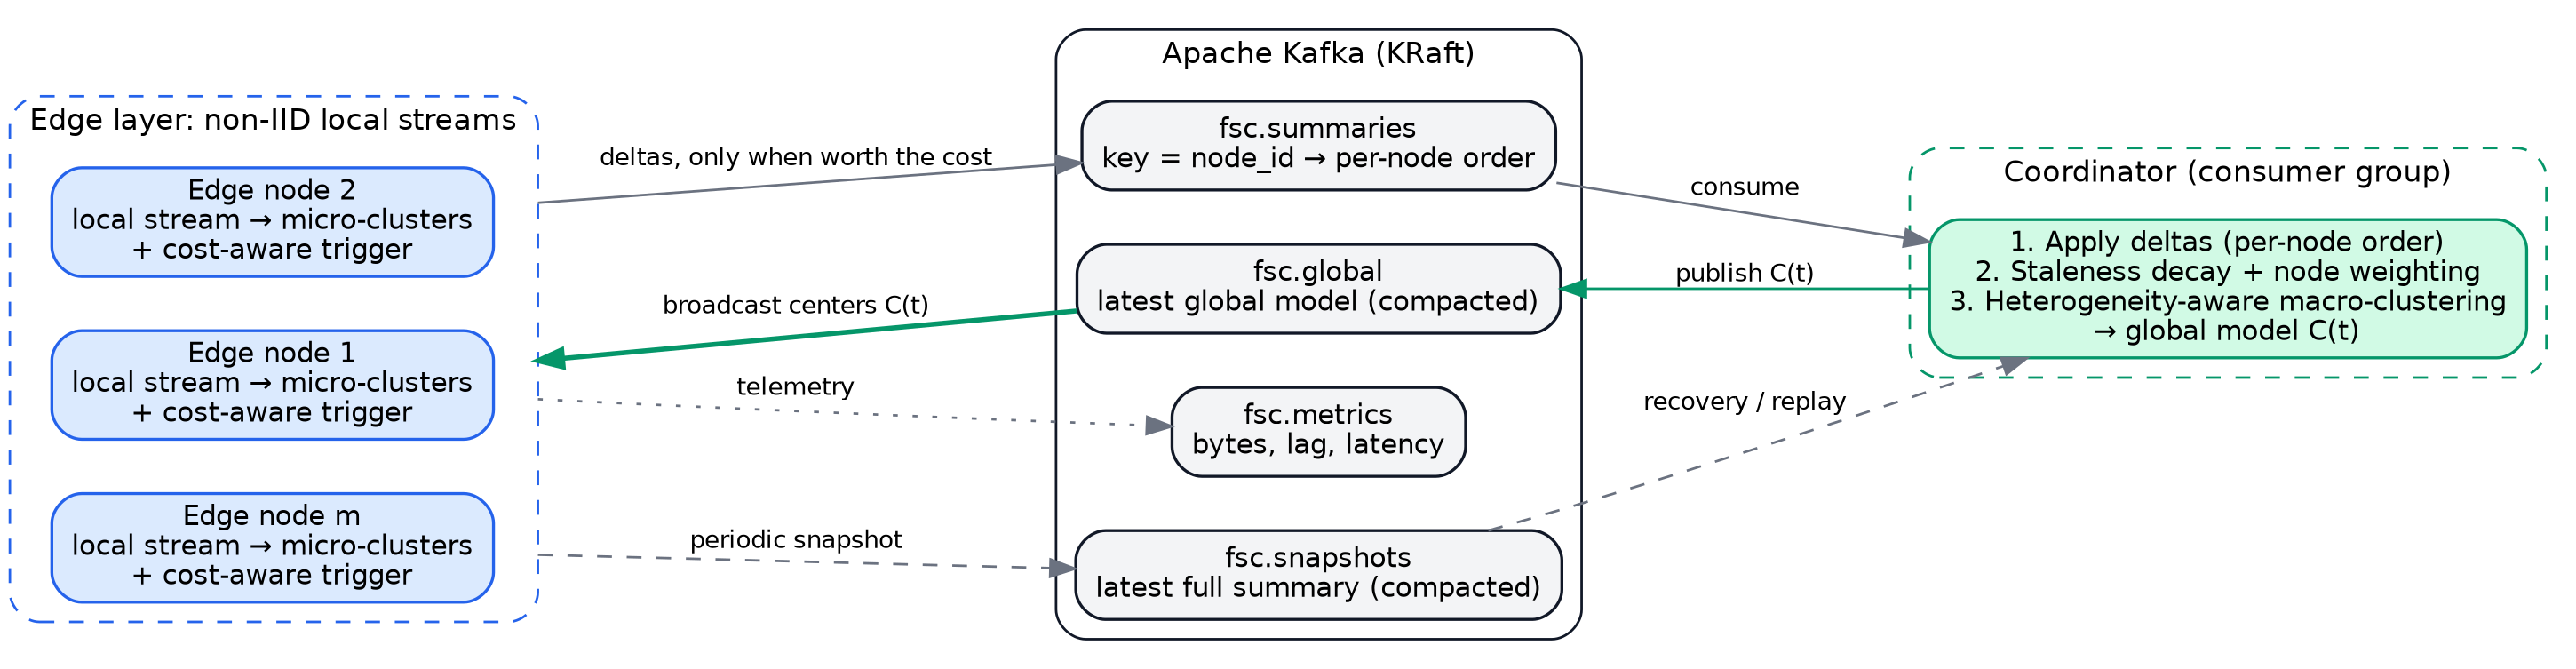
\includegraphics[width=0.92\textwidth]{../docs/figures/architecture.png}
\caption{FedCAST over Apache Kafka. Edge nodes publish prioritised CF deltas only when they are worth their byte cost. The coordinator applies them in per-node order, checkpoints its state to a compacted changelog, and broadcasts the global model on a compacted topic that the edges use to compute staleness.}\label{fig:arch}
\end{figure*}

Kafka~\cite{kreps2011kafka,wang2015kafkareplication} is not only the transport in FedCAST. Four of its semantics are part of the algorithm's correctness argument (Table~\ref{tab:kafka}).

\begin{table}[t]
\centering\small
\caption{Kafka semantics used by FedCAST.}\label{tab:kafka}
\begin{tabular}{@{}p{0.34\columnwidth}p{0.58\columnwidth}@{}}
\toprule
Semantics & Role in FedCAST\\
\midrule
Per-partition order, key $=$ node & Deltas of a node are applied in the order produced; a delta may assume its predecessor.\\
Idempotent producer + per-node sequence numbers & Retries on lossy links never double-apply a delta; replays after a crash are ignored.\\
Replayable log + committed offsets & A restarted coordinator replays only what it had not yet checkpointed; nodes never resend.\\
Log compaction & \texttt{fsc.snapshots} is a changelog holding one record per node (the server-side CFs and the offsets they reflect); \texttt{fsc.global} always holds the latest model, also for late joiners.\\
\bottomrule
\end{tabular}
\end{table}

\paragraph{Topics} \texttt{fsc.summaries} (8 partitions, key \texttt{node-}$i$) carries deltas. \texttt{fsc.snapshots} (compacted) is the coordinator's changelog. \texttt{fsc.global} (compacted, one partition) carries the model. \texttt{fsc.raw} is used only by the centralised baseline, and \texttt{fsc.metrics} carries telemetry.

\paragraph{Wire format} Messages use a fixed little-endian binary layout: a 20-byte header (kind, node, sequence number, time, counts, dimension) followed by packed arrays. The size of a pending delta is therefore known \emph{before} encoding, which the trigger~\eqref{eq:trigger} requires, and decoding is zero-copy. JSON would be 3--5$\times$ larger and of variable size. Avro or Protobuf would require a schema registry service.

\paragraph{Exactly-once state and recovery} The coordinator follows the state-store-plus-changelog pattern of stream processors~\cite{carbone2017flinkstate}. Every few seconds it writes, per node, a full CF record to \texttt{fsc.snapshots}, with the last applied sequence number and the \texttt{fsc.summaries} offsets as record headers, and then commits the offsets. On restart it reads the compacted changelog, restores all node states, and resumes \texttt{fsc.summaries} at the checkpointed offsets. Records after the checkpoint are applied again, and any record at or below a node's restored sequence number is ignored. The recovered state is therefore identical to that of an uninterrupted coordinator (Section~\ref{sec:rq4}).

\paragraph{Low-memory deployment} The broker runs in KRaft mode (no ZooKeeper) with a 256\,MB heap. We measured 317\,MB idle and 423\,MB peak RSS under a 300k-message load test; in Docker with a 512\,MB cap it never ran out of memory. All simulated nodes share one Python process ($\approx$150\,MB) with one idempotent producer each, and the coordinator needs $\approx$140\,MB. The complete system runs in under 1\,GB of RAM, which makes it reproducible on commodity laptops without Flink or Spark.

\paragraph{Two execution modes, one code base} The same \texttt{EdgeNode}, policy, codec and coordinator classes run (i) against a real broker and (ii) inside a deterministic discrete-event simulator. The simulator replaces the broker with seeded per-node links (delay, jitter, bandwidth cap, loss with retransmission, outages) that preserve per-key FIFO order and count retransmitted bytes. The simulator enables thousands of seeded runs. The Kafka mode provides the systems measurements and validates the simulator's byte accounting against Kafka's producer statistics.

\section{Experimental setup}\label{sec:setup}

\paragraph{Research questions} \textbf{RQ1} How much communication does FedCAST save at equal clustering quality, and what quality does it achieve at equal byte budgets? \textbf{RQ2} How does quality depend on the degree of statistical heterogeneity? \textbf{RQ3} How fast does the global model react to drift and to newly emerging clusters? \textbf{RQ4} How robust is the system to heterogeneous links, outages, and coordinator or broker failures? \textbf{RQ5} How does it scale with the number of nodes?

\paragraph{Datasets} Labels are used for evaluation only. \emph{SynDrift} is our seeded evolving stream: 60k points in $d{=}10$ from $k{=}15$ anisotropic Gaussians with random orientation, per-axis scales in $[0.3,1.5]$ and Dirichlet(2) sizes. Four clusters drift by 5 units, two clusters emerge at 35\,\% and 65\,\% of the stream, and one vanishes at 50\,\%. \emph{NSL-KDD}~\cite{tavallaee2009nslkdd}: network-intrusion records with 5 classes (normal, DoS, probe, R2L, U2R). We log-transform the 38 numeric features and one-hot encode protocol and flag, giving 51 features; we use a random sample of 60k of the 126k records. \emph{Shuttle}, \emph{Pen-Digits} and \emph{Letter} come from PMLB~\cite{olson2017pmlb}: 58k$\times$9 with 7 classes and 78\,\% majority, 11k$\times$16 with 10 classes, and 20k$\times$16 with 26 classes. Features are standardised.

\paragraph{Streams and partitions} The data are split across $m{=}10$ nodes and replayed over 300\,s of stream time with a 1\,s tick. Partitions: IID; Dirichlet($\alpha$) label skew~\cite{hsu2019noniid} with $\alpha\in\{1,0.3,0.1\}$ (default $0.3$); cluster-exclusive nodes that hold $k'\in\{2,1\}$ classes (the regime of~\cite{dennis2021kfed}); and \emph{class-rotation drift}, where at 50\,\% of the stream every node switches to the classes of its neighbour.

\paragraph{Network} Nodes alternate between a WAN link (80\,ms delay, 1\,\% loss, 5\,Mbit/s) and a cellular link (150\,ms, 3\,\%, 1\,Mbit/s). RQ4 adds LAN and poor links (300\,ms, 8\,\%, 128\,kbit/s) and 45\,s outages on three nodes. Lost messages are retransmitted after a 300\,ms timeout, and the retransmitted bytes are counted as wire bytes.

\paragraph{Baselines} All baselines share FedCAST's local micro-clusterer and aggregator, so differences come from \emph{what and when} each node sends:
\emph{Centralised-Raw} streams every point through Kafka to one server-side micro-clusterer with $mq$ slots, giving the quality upper bound;
\emph{Naive} sends the full summary whenever it changed;
\emph{Periodic} sends the full summary every $T$ seconds, as in classic federated rounds~\cite{mcmahan2017fedavg};
\emph{Periodic-$\Delta$} sends only the changed micro-clusters every $T$ seconds;
\emph{Change-Threshold} sends micro-clusters that were created, deleted, or changed by more than $\varepsilon$ relative to their radius or weight~\cite{tran2013communication,gama2011dgclust};
\emph{Norm-Trigger} sends changed micro-clusters when the relative norm of the summary change exceeds $\delta$~\cite{ghosh2021eventgrad};
\emph{k-FED}~\cite{dennis2021kfed} sends $k'$ local centres, as exact CF sums, every $T$ seconds, with the oracle number of local classes as $k'$.
We sweep each method's knob: $T\in\{15,\dots,240\}$\,s, $\varepsilon\in\{0.3,1,3\}$, $\delta\in\{0.05,0.2,0.5\}$, and FedCAST budgets $B/W\in\{5,\dots,500\}$\,B/s per node.

\paragraph{FedCAST settings} $q{=}50$, $H{=}120$\,s, $r_\text{mult}{=}2$, $r_\text{min}{=}0.25$; $\gamma{=}0.9$, $\rho{=}1$, $\eta{=}0.5$, $W{=}10$\,s; aggregation every 5\,s with 3 swaps and 2 restarts; $k$ equals the number of classes. The same values are used for every dataset; sensitivity is reported in Section~\ref{sec:ablation}.

\paragraph{Metrics} Every 10\,s the server's current model labels the points of the last 60\,s, up to 3000 points. We report the \emph{cost ratio}, the k-means cost of the server model divided by that of Centralised-Raw on the same seed (the objective FedCAST controls; lower is better), together with ARI~\cite{hubert1985ari}, NMI, purity and per-class recall. Cost is measured in uplink bytes: payload plus a 24-byte per-record Kafka overhead, which is validated against Kafka's producer statistics in Section~\ref{sec:rq4}. Averages exclude the first 10\,\% of the stream.

\paragraph{Statistical protocol} Each configuration is run with 5 seeds, which vary the partition, the stream order, the links and the aggregation. For budget-matched comparisons we interpolate every method's (bytes, quality) curve per seed at 1\,\%, 3\,\% and 10\,\% of Centralised-Raw's bytes, in log-bytes, keeping the best quality attainable within the budget. A method that cannot operate at a budget is marked infeasible. We use the Friedman test with the Nemenyi critical difference over dataset$\times$budget blocks, and one-sided Wilcoxon signed-rank tests with Holm correction~\cite{demsar2006statistical}.

\paragraph{Implementation} Python 3.11, NumPy, scikit-learn and confluent-kafka (librdkafka); Apache Kafka 3.8 in KRaft mode. All runs used one 4-core machine; the complete system also runs on a laptop with under 1\,GB of RAM.

\section{Results}\label{sec:results}
\subsection{RQ1: Communication versus quality}\label{sec:rq1}

\begin{figure*}[t]
\centering
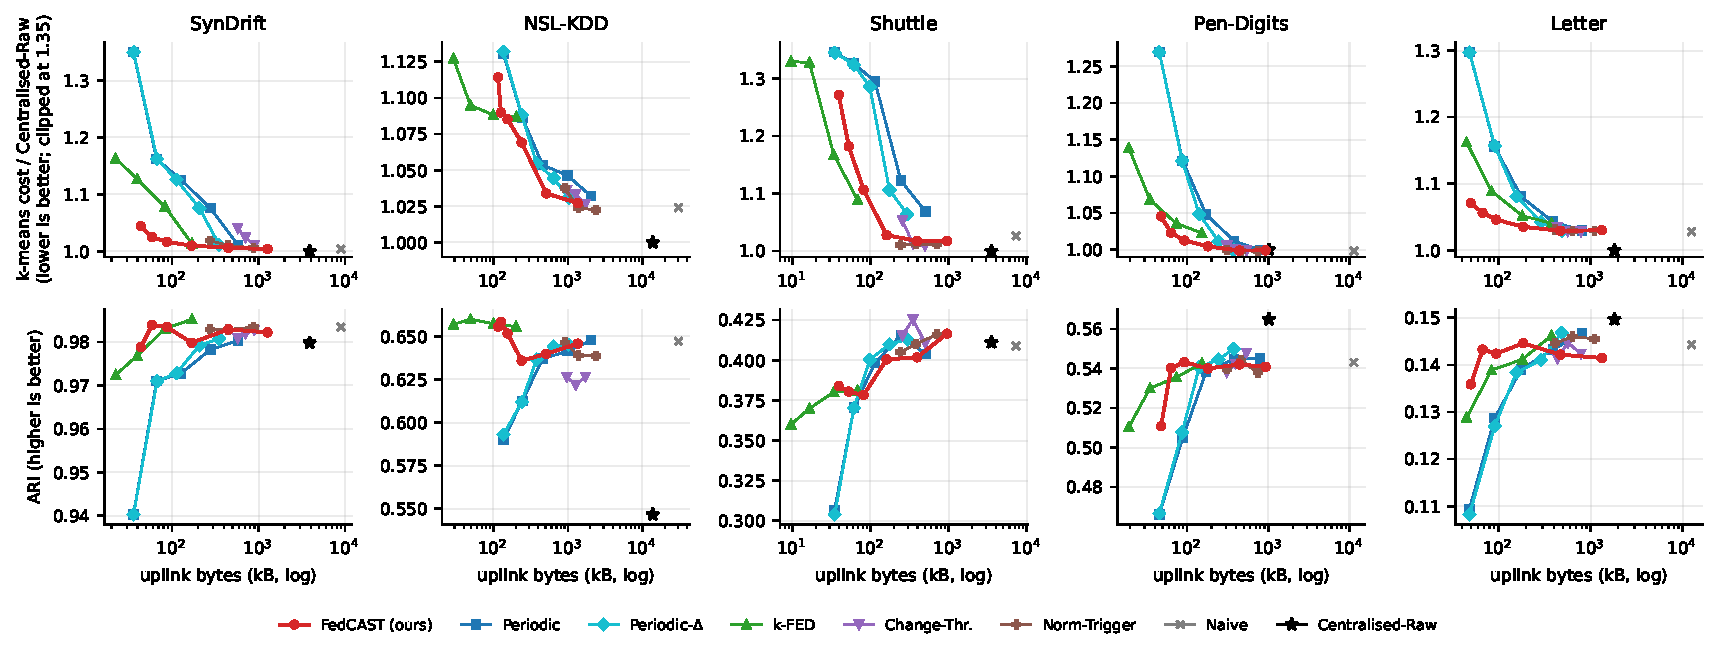
\includegraphics[width=\textwidth]{fig_pareto}
\caption{Cost--quality trade-off on five datasets (mean of 5 seeds; each marker is one parameter setting). Top: k-means cost of the server's model relative to Centralised-Raw (lower is better). Bottom: ARI. FedCAST (red) dominates across the practically relevant range. k-FED is cheaper at the extreme low end on well-separated data. Change- and Norm-triggered reporting cannot operate below a data-dependent byte floor.}\label{fig:pareto}
\end{figure*}

Figure~\ref{fig:pareto} shows the Pareto fronts. FedCAST's front lies at or below every baseline from about 1.5\,\% of the Centralised-Raw traffic upward, on all five datasets. Table~\ref{tab:savings} quantifies the gap as the bytes each method needs to bring the cost within 5\,\% of the centralised learner. FedCAST needs \textbf{10--61\,\% fewer bytes than the best baseline} on each dataset, and \textbf{1.8--8.5$\times$ fewer than Periodic}. Some baselines never reach this quality within their parameter range: k-FED on NSL-KDD and Shuttle, and Periodic on Shuttle.

\begin{table}[t]
\centering\small
\caption{Uplink kB needed to reach a cost ratio $\le1.05$ (mean curve, log-interpolated). ``--'': not reached.}\label{tab:savings}
\setlength{\tabcolsep}{3pt}
\begin{tabular}{@{}lrrrrrrr@{}}
\toprule
 & \textbf{FedCAST} & Per. & Per.-$\Delta$ & k-FED & Chg. & Norm & saving\\
\midrule
SynDrift & \textbf{44} & 372 & 256 & 113 & 574 & 276 & 61\,\%\\
NSL-KDD & \textbf{362} & 668 & 484 & -- & 969 & 907 & 25\,\%\\
Shuttle & \textbf{133} & -- & -- & -- & 263 & 242 & 45\,\%\\
Pen-Digits & \textbf{48} & 169 & 140 & 53 & 309 & 309 & 10\,\%\\
Letter & \textbf{83} & 334 & 256 & 204 & 435 & 412 & 60\,\%\\
\bottomrule
\end{tabular}
\end{table}

\begin{table}[t]
\centering\small
\caption{Budget-matched cost ratio (lower is better; mean of 5 seeds) at 1/3/10\,\% of Centralised-Raw bytes. ``--'': the method cannot operate within that budget. Rows where no method is feasible are omitted.}\label{tab:matched}
\setlength{\tabcolsep}{2.4pt}
\begin{tabular}{@{}llrrrrrr@{}}
\toprule
Data & Bud. & \textbf{FedCAST} & Per. & Per.-$\Delta$ & k-FED & Chg. & Norm\\
\midrule
\multirow{3}{*}{SynDrift} & 1\% & -- & 2.796 & 2.813 & \textbf{1.128} & -- & --\\
 & 3\% & \textbf{1.013} & 1.130 & 1.123 & 1.047 & -- & --\\
 & 10\% & \textbf{1.007} & 1.046 & 1.011 & 1.013 & -- & 1.012\\
\multirow{3}{*}{NSL-KDD} & 1\% & 1.084 & 1.157 & 1.158 & \textbf{1.082} & -- & --\\
 & 3\% & \textbf{1.043} & 1.059 & 1.053 & 1.078 & -- & --\\
 & 10\% & 1.027 & 1.039 & 1.031 & 1.078 & 1.030 & \textbf{1.025}\\
\multirow{3}{*}{Shuttle} & 1\% & -- & 1.354 & 1.355 & \textbf{1.161} & -- & --\\
 & 3\% & \textbf{1.076} & 1.297 & 1.263 & 1.089 & -- & --\\
 & 10\% & 1.012 & 1.095 & 1.064 & 1.089 & 1.013 & \textbf{1.003}\\
\multirow{2}{*}{Pen-Dig.} & 3\% & -- & -- & -- & \textbf{1.084} & -- & --\\
 & 10\% & \textbf{1.011} & 1.105 & 1.097 & 1.030 & -- & --\\
\multirow{2}{*}{Letter} & 3\% & \textbf{1.067} & 1.270 & 1.271 & 1.139 & -- & --\\
 & 10\% & \textbf{1.036} & 1.079 & 1.072 & 1.052 & -- & --\\
\bottomrule
\end{tabular}
\end{table}

Table~\ref{tab:matched} compares methods at equal budgets. Among the methods that can operate at small budgets (FedCAST, Periodic, Periodic-$\Delta$, k-FED), FedCAST obtains the lowest mean Friedman rank over the 10 dataset$\times$budget blocks where all four are feasible: 1.1, against 2.5 for k-FED, 2.8 for Periodic-$\Delta$ and 3.6 for Periodic. The Friedman test gives $\chi^2{=}19.6$, $p{=}2.1{\times}10^{-4}$ (Figure~\ref{fig:cd}). One-sided Wilcoxon tests over all paired seeds confirm the ordering after Holm correction: FedCAST beats Periodic ($p{=}3.5{\times}10^{-13}$, wins 96\,\% of pairs), Periodic-$\Delta$ ($p{=}5.4{\times}10^{-11}$, 94\,\%) and k-FED ($p{=}1.7{\times}10^{-9}$, 88\,\%). At 10\,\% of raw traffic, the change- and norm-triggered baselines become feasible and are within about 1\,\% of FedCAST, but they need 3--20$\times$ more bytes to get there (Table~\ref{tab:savings}). Two regimes favour k-FED: the very lowest budgets (1\,\%) and the small, well-separated Pen-Digits stream. There, a single message of $k'$ centres is cheaper than FedCAST's bootstrap summary of $q$ micro-clusters. This is a genuine limitation that we discuss in Section~\ref{sec:discussion}.

\begin{figure}[t]
\centering
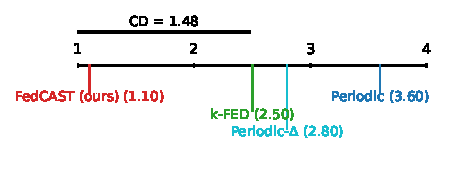
\includegraphics[width=0.9\columnwidth]{fig_cd}
\caption{Critical-difference diagram (Nemenyi, $\alpha{=}0.05$) of mean ranks by budget-matched cost ratio.}\label{fig:cd}
\end{figure}

Byte counts are credible. On a real broker, our per-message estimate (payload plus 24\,B record overhead) exceeded librdkafka's \texttt{txmsg\_bytes} by only 0.7--3.0\,\% for every method (Table~\ref{tab:k1}), so all reported savings are conservative.

\subsection{RQ3: Drift and emerging clusters}\label{sec:rq3}

\begin{figure*}[t]
\centering
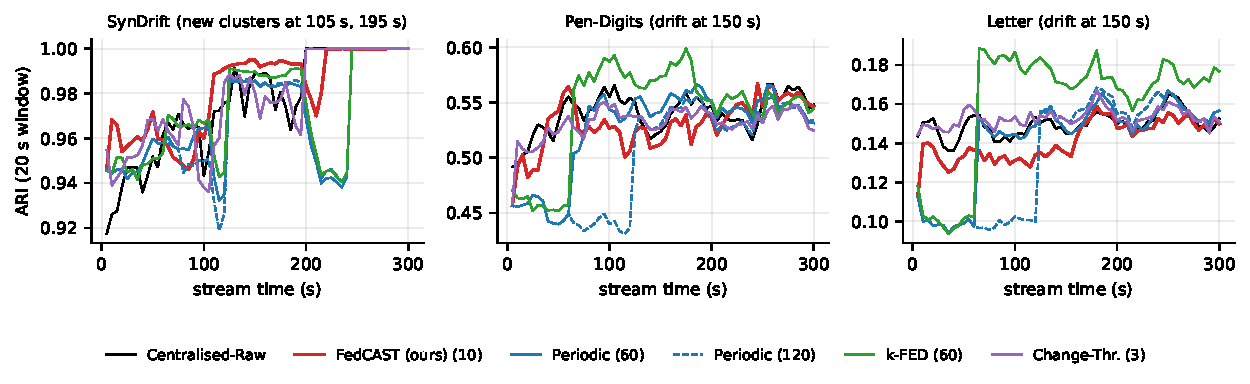
\includegraphics[width=\textwidth]{fig_drift}
\caption{ARI over time (20\,s window, mean of 5 seeds). On SynDrift, new clusters emerge at 105\,s and 195\,s at few nodes. FedCAST (10\,B/s per node, 59\,kB total) picks them up about 2.5$\times$ faster than Periodic and k-FED, while sending less than Periodic-60 (127\,kB). On Pen-Digits and Letter, node class sets rotate at 150\,s.}\label{fig:drift}
\end{figure*}

On SynDrift (Figure~\ref{fig:drift}, left), the novelty override and the objective-linked trigger let FedCAST report each emerging cluster as soon as enough mass has accumulated. The mean delay until an emerging class is recalled at $\ge50\,\%$ is $10.9\pm5.6$\,s at 10\,B/s and $9.4\pm2.6$\,s at 20\,B/s, against 27.4\,s for Periodic-60, Periodic-120, Periodic-$\Delta$ and k-FED. It does so with 59--87\,kB of uplink, compared with 113--127\,kB for the 60\,s periodic variants. Change-Threshold reacts within one evaluation interval (4.9\,s) but spends 574\,kB, almost 10$\times$ more. The cost ratio over the whole evolving stream is 1.027--1.043 for FedCAST, against 1.23--1.27 for the periodic methods and k-FED. Under class-rotation drift, which changes \emph{which node} sees a class but not the global mixture, all methods keep a valid model. FedCAST again pairs the lowest traffic with a lower cost than Periodic (Pen-Digits: 1.013 at 96\,kB against 1.042 at 173\,kB).

\paragraph{The budget is respected} Figure~\ref{fig:budget} shows every node's cumulative spend. After the one-time bootstrap summary, which is paid from the token bucket's initial allowance $\kappa$, the slope equals the configured budget: 10.0 and 18\,B/s for $B/W{=}10$ and 20. No node ever crosses the hard envelope $\kappa+Bt$ of Proposition~\ref{prop:budget}.

\begin{figure}[t]
\centering
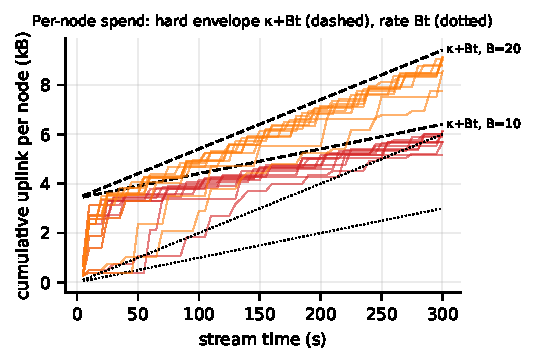
\includegraphics[width=0.85\columnwidth]{fig_budget}
\caption{Per-node cumulative uplink for FedCAST on SynDrift with $B/W=10$ and $20$\,B/s (all 10 nodes). Dashed: the hard envelope $\kappa+Bt$; dotted: the rate $Bt$.}\label{fig:budget}
\end{figure}

\subsection{RQ2: Degree of statistical heterogeneity}\label{sec:rq2}

\begin{figure*}[t]
\centering
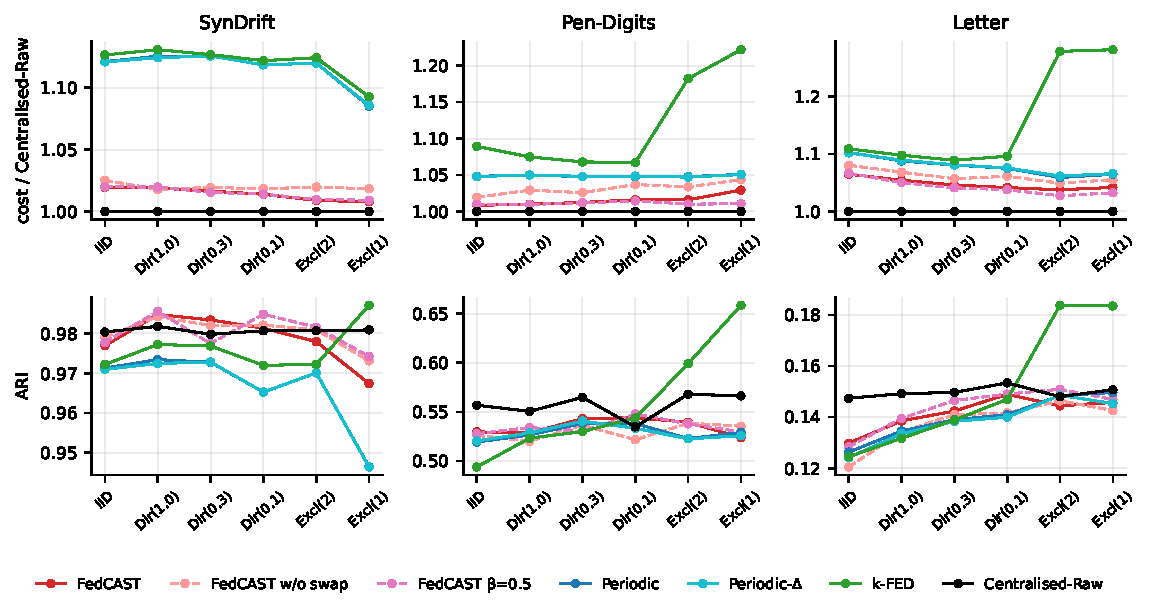
\includegraphics[width=0.9\textwidth]{fig_noniid}
\caption{Quality as heterogeneity grows, from IID through Dirichlet label skew to cluster-exclusive nodes (Excl($k'$): each node holds $k'$ classes). FedCAST at 20\,B/s per node against Periodic-60, Periodic-$\Delta$-60 and k-FED-60 (similar or larger traffic), with two aggregator variants. Mean of 5 seeds.}\label{fig:noniid}
\end{figure*}

Figure~\ref{fig:noniid} varies the partition from IID to cluster-exclusive nodes. FedCAST attains the lowest cost ratio in all 18 combinations of dataset and partition: 1.008--1.065, against 1.047--1.126 for Periodic and Periodic-$\Delta$ and 1.067--1.281 for k-FED. Its quality does not degrade with heterogeneity. On SynDrift it even improves, from 1.019 (IID) to 1.008 (one class per node), because exclusive clusters produce concentrated, high-value deltas.

\paragraph{Aggregator} Swap local search lowers the cost in 17 of 18 settings (e.g.\ Pen-Digits Dir(0.1): 1.016 against 1.037 without swaps). Node balancing ($\beta{=}0.5$) is neutral under mild skew but helps in the cluster-exclusive regime (Pen-Digits Excl(1): 1.011 against 1.029; Letter Excl(2): 1.027 against 1.038). There, a node with a large share of the traffic would otherwise pull several centres towards its own clusters.

\paragraph{k-FED's regime} With one or two classes per node and the oracle $k'$, k-FED reaches the highest \emph{label} agreement (Pen-Digits Excl(1): ARI 0.66 against 0.52--0.57 for all other methods, including Centralised-Raw), consistent with its theory~\cite{dennis2021kfed}. Its k-means cost, however, is 22\,\% above the centralised learner. Each local centre equals a class mean, so k-FED recovers the class partition rather than the k-means optimum. When labels are the goal and each node holds few, well-separated classes, k-FED's one-centre-per-class summaries are an excellent choice. When the goal is a faithful global clustering objective, FedCAST is.

\subsection{Ablations}\label{sec:ablation}

\begin{table}[t]
\centering\small
\caption{Ablation of FedCAST components at 20\,B/s per node: cost ratio (lower is better, mean of 5 seeds) and mean uplink.}\label{tab:ablation}
\setlength{\tabcolsep}{2.6pt}
\begin{tabular}{@{}lrrrrrr@{}}
\toprule
Variant & Syn & KDD & Shut. & Pen & Let. & kB\\
\midrule
\textbf{FedCAST} & \textbf{1.016} & \textbf{1.085} & 1.107 & 1.012 & 1.046 & 102\\
w/o prioritisation ($\gamma{=}1$) & 1.333 & 1.132 & 1.331 & 1.035 & 1.061 & 87\\
full summaries & 1.295 & 1.132 & 1.321 & 1.037 & 1.054 & 89\\
w/o swap search & 1.019 & 1.101 & 1.218 & 1.026 & 1.057 & 102\\
w/o dual ascent & 1.019 & 1.088 & 1.108 & 1.011 & 1.047 & 102\\
w/o link price & 1.017 & 1.090 & \textbf{1.065} & 1.012 & \textbf{1.044} & 103\\
w/o novelty & 1.017 & 1.090 & 1.092 & 1.012 & 1.047 & 102\\
w/o server decay & 1.017 & 1.089 & 1.106 & \textbf{1.011} & 1.047 & 102\\
\bottomrule
\end{tabular}
\end{table}

Table~\ref{tab:ablation} isolates each component at a fixed budget. \emph{Prioritised partial deltas are the single most important ingredient.} Sending all dirty micro-clusters ($\gamma{=}1$) or full summaries raises the cost by up to 32\,\% on SynDrift and 22\,\% on Shuttle. Under the same budget, large messages drain the token bucket, so sends become rare. Prioritisation spends the same bytes on the few micro-clusters that actually move the objective. Swap search is the second most important component (Shuttle: 1.107 against 1.218 without it). The remaining components leave the \emph{average} cost at this budget essentially unchanged, because their purpose lies elsewhere. The novelty override targets \emph{reaction time} to new clusters, the link price targets \emph{wire cost} on bad links, and dual ascent targets \emph{loose} budgets, where it prevents spending bytes on updates that carry no value. Section~\ref{sec:rq4} and Table~\ref{tab:targeted} evaluate these targeted effects. Removing the link price even lowers the cost slightly on Shuttle and Letter: the price deliberately shifts traffic away from expensive links at a small quality cost.

\subsection{RQ4: Network heterogeneity, outages and failures}\label{sec:rq4}

\paragraph{Heterogeneous links and outages} Table~\ref{tab:net} runs every method under three network scenarios: homogeneous WAN; heterogeneous LAN/WAN/cellular/poor links; and the same with 45\,s outages at three nodes. Kafka-style retries and buffering deliver every summary eventually, and the coordinator's staleness decay stops silent nodes from freezing stale mass. As a result, every method's quality is nearly unchanged across scenarios. FedCAST's cost ratio moves by at most 0.009 (SynDrift 1.015--1.017, NSL-KDD 1.071--1.080), and retransmissions add only 1--3\,\% wire bytes. The ordering between methods is the same as in RQ1.

\begin{table}[t]
\centering\small
\caption{Cost ratio (uplink kB) under network scenarios; mean of 5 seeds.}\label{tab:net}
\setlength{\tabcolsep}{2.5pt}
\begin{tabular}{@{}llrrr@{}}
\toprule
Data & Method & homog.\ WAN & hetero & hetero+outage\\
\midrule
\multirow{5}{*}{SynDrift} & \textbf{FedCAST} & \textbf{1.015} (87) & \textbf{1.016} (87) & \textbf{1.017} (85)\\
 & Periodic-60 & 1.125 (127) & 1.125 (127) & 1.126 (127)\\
 & Periodic-$\Delta$-60 & 1.126 (113) & 1.125 (113) & 1.126 (113)\\
 & k-FED-60 & 1.127 (40) & 1.126 (40) & 1.127 (40)\\
 & Change-Thr. & 1.040 (574) & 1.040 (574) & 1.041 (574)\\
\midrule
\multirow{5}{*}{NSL-KDD} & \textbf{FedCAST} & 1.071 (154) & 1.077 (156) & 1.080 (156)\\
 & Periodic-60 & 1.048 (459) & 1.050 (459) & 1.058 (459)\\
 & Periodic-$\Delta$-60 & 1.048 (379) & 1.048 (379) & 1.058 (379)\\
 & k-FED-60 & 1.084 (49) & 1.085 (49) & 1.084 (49)\\
 & Change-Thr. & \textbf{1.028} (969) & \textbf{1.027} (969) & \textbf{1.027} (969)\\
\bottomrule
\end{tabular}
\end{table}

\paragraph{What the remaining components are for} Table~\ref{tab:targeted} tests the three components whose average-cost effect in Table~\ref{tab:ablation} was negligible, each on the metric it is designed for. (i) \emph{Link price.} Under loose budgets on heterogeneous links, the price shifts 4--7\,\% of the traffic away from cellular and poor links and saves 3\,\% of wire bytes at unchanged quality. At tight budgets (Table~\ref{tab:net}) it has no effect, because the token bucket, not the threshold, is the binding constraint. (ii) \emph{Dual ascent.} Under a loose budget it makes the spend track the budget (62--85\,\% used, against 30--36\,\% with $\lambda$ frozen at its initial value) without changing quality. This shows it is the mechanism that makes $B$, rather than an arbitrary $\lambda_0$, the operating knob. It also shows that beyond some budget, extra bytes buy nothing, which suggests a value floor as a refinement. (iii) \emph{Novelty override.} Detection delays are identical with and without it (10.9 and 9.4\,s). The objective-linked score alone already reacts to emerging clusters, because a new micro-cluster far from every centre carries a large cost term. The override is therefore a redundant safety net, and we keep it only for its small cost benefit at the tightest budget (1.051 against 1.060).

\begin{table}[t]
\centering\small
\caption{Targeted ablations: each component on the metric it is designed for (mean of 5 seeds).}\label{tab:targeted}
\setlength{\tabcolsep}{2pt}
\resizebox{\columnwidth}{!}{%
\begin{tabular}{@{}llrl@{}}
\toprule
Component & Setting & on / off & target metric (on vs.\ off)\\
\midrule
Link price & Syn, 500\,B/s & 1276 / 1321 kB & bad/good-link bytes 0.93 vs 0.97\\
 & KDD, 500\,B/s & 1371 / 1414 kB & bad/good-link bytes 0.99 vs 1.04\\
Dual ascent & Syn, 500\,B/s & 1.004 / 1.007 & budget used 85\,\% vs 36\,\%\\
 & Pen, 500\,B/s & 0.999 / 0.999 & budget used 62\,\% vs 30\,\%\\
Novelty & Syn, 10\,B/s & 1.051 / 1.060 & detection 10.9\,s vs 10.9\,s\\
 & Syn, 20\,B/s & 1.035 / 1.035 & detection 9.4\,s vs 9.4\,s\\
\bottomrule
\end{tabular}}
\end{table}


\paragraph{Coordinator crash (real Kafka)} We ran 10 edge nodes with FedCAST against two coordinators in different consumer groups: a \emph{shadow} that never fails and a \emph{victim} that we kill with SIGKILL after 15\,s (no clean shutdown, no final checkpoint) and restart 8\,s later. The restarted victim rebuilt all 10 node states from the compacted changelog in 1.08\,s, resumed \texttt{fsc.summaries} at the checkpointed offsets, and caught up within 0.5\,s. At the end of the run its state was \emph{identical} to the shadow's: the same micro-cluster identifiers for every node and a maximum node-mass difference of 0.0. All 238 summaries were applied exactly once, and no node resent anything.

\paragraph{Broker outage (real Kafka)} We stopped the Kafka broker in the middle of a run for 34\,s. The idempotent producers buffered and retried, and after the restart all 231 summaries sent by the nodes were applied by the coordinator: zero lost, zero delivery errors.

\begin{table}[t]
\centering\small
\caption{Byte accounting on a real broker: our per-message estimate (payload + 24\,B) against librdkafka's \texttt{txmsg\_bytes}.}\label{tab:k1}
\setlength{\tabcolsep}{3pt}
\begin{tabular}{@{}lrrr@{}}
\toprule
Method & estimate (B) & Kafka (B) & difference\\
\midrule
FedCAST 20 B/s & 55{,}978 & 54{,}340 & $+3.0\,\%$\\
FedCAST 150 B/s & 230{,}798 & 226{,}028 & $+2.1\,\%$\\
Periodic 30\,s & 189{,}160 & 187{,}900 & $+0.7\,\%$\\
Periodic-$\Delta$ 30\,s & 153{,}264 & 152{,}004 & $+0.8\,\%$\\
k-FED 30\,s & 57{,}760 & 56{,}500 & $+2.2\,\%$\\
Centralised-Raw & 2{,}486{,}473 & 2{,}450{,}275 & $+1.5\,\%$\\
\bottomrule
\end{tabular}
\end{table}

\subsection{RQ5: Scalability and footprint}\label{sec:rq5}

\begin{figure}[t]
\centering
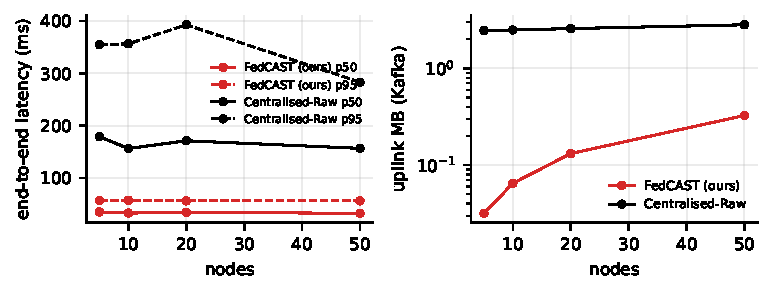
\includegraphics[width=\columnwidth]{fig_kafka_scale}
\caption{Real Kafka, 5--50 nodes on one 4-core machine: end-to-end latency from produce to coordinator consumption (left) and total uplink bytes (right, log scale).}\label{fig:kscale}
\end{figure}

Figure~\ref{fig:kscale} scales the real deployment from 5 to 50 edge nodes, each with its own idempotent producer, streaming 60k points in 20\,s of wall time (about 1{,}900 points/s). FedCAST's end-to-end latency stays flat at 33--35\,ms (p50) and 57\,ms (p95) at every scale, because nodes send few and small messages. Centralised-Raw's latency is 4--5$\times$ higher (156--179\,ms p50, 283--393\,ms p95) while it ships 2.5--2.8\,MB, against 32--325\,kB for FedCAST. FedCAST's traffic grows linearly with the number of nodes (6.5\,kB per node for 200\,s of stream), as the per-node budget prescribes. Quality is unchanged (ARI 0.97--0.99). The simulated scaling experiment agrees: bytes per node are constant and ARI stays within 0.97--0.99 from 5 to 50 nodes (Periodic: 0.95--0.98). Memory stays small. At 50 nodes the edge process needs 172\,MB, the coordinator 141\,MB and the broker 475\,MB, 788\,MB in total, which confirms that the complete system runs on a commodity laptop.



\section{Discussion}\label{sec:discussion}

\paragraph{When to use which method} FedCAST pays off whenever the byte budget is tight relative to how fast the data evolves: it spends bytes where the global objective is affected and when it is affected. When budgets are generous (above roughly 10\,\% of the bytes of sending raw data), every event-driven method converges to the centralised quality, and the choice among them matters little. k-FED is extremely frugal when clusters are well separated and each node holds few of them, exactly the regime its theory covers~\cite{dennis2021kfed}. It needs the local $k'$ (we gave it the oracle value), carries no shape information, and reacts only at its period, so it degrades on overlapping, drifting or imbalanced data. Change- and norm-triggered reporting reaches good quality but cannot be run below a data-dependent byte floor, and its thresholds must be re-tuned per dataset. FedCAST instead takes the budget itself as input.

\paragraph{What matters in FedCAST} The ablations separate the essential from the auxiliary. Prioritised partial deltas, together with an objective-linked score to rank them, deliver most of the gain: the budget is spent on the few micro-clusters that move the objective. Swap search matters under heterogeneity. The dual-ascent threshold turns the byte budget into the operating knob. The link price redistributes traffic only when budgets are loose. The novelty override turned out to be redundant with the objective-linked score. We report this negative result because it simplifies deployment: the score alone suffices to react to emerging clusters.

\paragraph{Kafka as part of the algorithm} Designing the protocol around Kafka's semantics removed whole classes of failure handling from the algorithm. Deltas can assume their predecessor because of per-key order. Retransmissions are harmless because of idempotence and sequence numbers. Nodes never resend after a server crash because of replay and a compacted changelog. Late joiners and restarted nodes obtain the model from the compacted \texttt{fsc.global}. The price is a broker, which runs in about 400\,MB.

\paragraph{Privacy} CFs reveal aggregate statistics (counts, sums, sums of squares) rather than records. They are not differentially private. Adding calibrated Gaussian noise to each delta after clipping $\lVert x\rVert$ is a natural extension~\cite{epasto2023dpstream}. The budget controller then also bounds the number of releases, and hence the privacy composition. We leave this three-way trade-off between bytes, accuracy and privacy to future work.

\paragraph{Limitations and threats to validity} (i) Scale: experiments emulate up to 50 nodes on one machine, with real Kafka for systems metrics and a validated simulator for sweeps. Wide-area deployments add effects such as cross-region replication that we do not model. (ii) Label-based metrics on real data are bounded by how well classes form k-means clusters (e.g.\ Shuttle, Letter). We therefore report the cost ratio to a centralised learner, which is the objective every method optimises. (iii) The macro-clustering assumes $k$ is known; an unknown-$k$ aggregator such as AFCL~\cite{zhang2025afcl} or density-based aggregation could replace it without changing the send policy. (iv) Data rates are replayed in stream time, so wall-clock effects of real devices (CPU contention, energy) are measured only through the Kafka experiments. (v) At the very lowest budgets (about 1\,\% of raw traffic), FedCAST cannot operate, because its bootstrap summary of $q$ micro-clusters exceeds the budget, while k-FED's $k'$ centres fit. Letting the trigger operate on compressed summaries (fewer, merged micro-clusters) would close this gap.


\section*{Code and data availability}
All code, experiment configurations, raw results and scripts that regenerate every figure and table are available in the project repository. All datasets are public.

\bibliographystyle{elsarticle-num}
\bibliography{references}

\appendix
\section{Proofs}\label{app:proofs}

\paragraph{Proof of Proposition~\ref{prop:cost}} Micro-clusters are assigned independently, so $J(S_i;C)=\sum_{\mathrm{id}}J(\mathrm{CF}_{\mathrm{id}};C)$, where an identifier absent from one of the two sets contributes $0$ on that side. Pairing the two sums by identifier and applying the triangle inequality gives
\[
|J(S_i;C)-J(\hat S_i;C)|=\Big|\sum_{\mathrm{id}}\big(J(\mathrm{CF}_{\mathrm{id}};C)-J(\widehat{\mathrm{CF}}_{\mathrm{id}};C)\big)\Big|\le\sum_{\mathrm{id}}\big|J(\mathrm{CF}_{\mathrm{id}};C)-J(\widehat{\mathrm{CF}}_{\mathrm{id}};C)\big| .
\]
Each summand is the first term of $e_{\mathrm{id}}$ in~\eqref{eq:eid}, and the second term is non-negative, so the sum is at most $\Delta_i$. Summing over nodes gives the network-wide statement. Both copies are decayed to the same time with the same factor per identifier (Section~\ref{sec:problem}), so an unchanged micro-cluster has $e_{\mathrm{id}}=0$. \qed

\paragraph{Proof of Proposition~\ref{prop:centroid}}
\[
c_j'-\hat c_j'=\frac{\mathbf{L}_j}{N_j}-\frac{\hat{\mathbf{L}}_j}{\hat N_j}=\frac{\mathbf{L}_j-\hat{\mathbf{L}}_j}{N_j}+\hat{\mathbf{L}}_j\Big(\frac1{N_j}-\frac1{\hat N_j}\Big)=\frac{\mathbf{L}_j-\hat{\mathbf{L}}_j}{N_j}+\hat c_j'\,\frac{\hat N_j-N_j}{N_j}.
\]
Hence $\lVert c_j'-\hat c_j'\rVert\le\big(\lVert\mathbf{L}_j-\hat{\mathbf{L}}_j\rVert+\lVert\hat c_j'\rVert\,|N_j-\hat N_j|\big)/N_j$. Because both sums run over the same identifiers $A_j$, the triangle inequality gives $\lVert\mathbf{L}_j-\hat{\mathbf{L}}_j\rVert\le\sum_{A_j}\lVert\mathbf{LS}_{\mathrm{id}}-\widehat{\mathbf{LS}}_{\mathrm{id}}\rVert$ and $|N_j-\hat N_j|\le\sum_{A_j}|n_{\mathrm{id}}-\hat n_{\mathrm{id}}|$. With $\lVert\hat c_j'\rVert\le\bar c_{\mathrm{id}}$, each summand is at most $e_{\mathrm{id}}/\rho$. \qed

\paragraph{Proof of Proposition~\ref{prop:budget}}
(i) A token bucket with rate $B_i/W$ and capacity $\kappa_i$ starts full, is never negative, and every send consumes its size. After time $T$ the total consumed is at most $\kappa_i+B_iT/W$.

(ii) Let $\theta_w=\log\lambda_w$ and $g_w=\mathrm{clip}_{[-1,2]}\big((\text{spent}_w-B_i)/B_i\big)$, so $\theta_{w+1}=\theta_w+\eta g_w$. Telescoping gives $\sum_{w\le n}g_w=(\theta_{n+1}-\theta_1)/\eta$. Next we bound $\theta$ from above. Every send satisfies $D_c\ge\lambda p_i b$ with $D_c\le\Delta_\text{max}$, $p_i\ge1$ and $b\ge b_\text{min}$. If $\lambda>\lambda^\dagger=\Delta_\text{max}/b_\text{min}$, no send can happen, so $\text{spent}_w=0$, $g_w=-1$, and $\theta$ decreases. Since one update raises $\theta$ by at most $2\eta$, $\theta_w\le\max(\theta_1,\log\lambda^\dagger)+2\eta$ for all $w$. Substituting, $\frac1n\sum_{w\le n}g_w\le\frac{\log(\lambda^\dagger e^{2\eta}/\lambda_0)}{\eta n}$, using $\theta_1=\log\lambda_0\le\log\lambda^\dagger$ w.l.o.g. The left-hand side is the average relative overspend, clipped at $2$; overspends larger than $2B_i$ in a window are already excluded by the bucket whenever $\kappa_i\le3B_i$. \qed

\end{document}
